\documentclass[11pt]{article}
\usepackage[a4paper,margin=1in]{geometry}
\usepackage[english]{babel}
\usepackage[T1]{fontenc}
\usepackage[utf8]{inputenc}
\usepackage{csquotes}
\usepackage{textcomp}
\usepackage[style=numeric,sorting=none,backend=biber]{biblatex}
\setcounter{biburllcpenalty}{100}
\setcounter{biburlucpenalty}{200}
\setcounter{biburlnumpenalty}{100}
\usepackage{setspace}
\usepackage{titlesec}
\usepackage{graphicx}
\usepackage{booktabs}
\usepackage{array}
\usepackage{amsmath}
\usepackage{amssymb}
\usepackage{enumitem}
\usepackage{tabularx}
\usepackage{hyperref}
\usepackage{xcolor}
\hypersetup{colorlinks=true,linkcolor=blue,urlcolor=blue,citecolor=blue}
\setstretch{1.15}

\addbibresource{references.bib}

\titleformat{\section}{\bfseries\large}{\thesection.}{0.5em}{}
\titleformat{\subsection}{\bfseries}{\thesubsection.}{0.5em}{}
\titleformat{\subsubsection}{\itshape}{\thesubsubsection.}{0.5em}{}

% ============================================================
% AI AND ETHICS — AUTHORED (NON-ANONYMIZED) VERSION
% This is the master source-of-truth manuscript with full
% author identity. The anonymized variant for SNAPP submission
% strips the author block, MIT/CESAR affiliations, ORCID, and
% identifying remarks. Use main_aie.tex for SNAPP uploads.
% ============================================================

\title{\textbf{A Data-Centric Trust Pipeline:\\An Empirical Framework for Trustworthy AI in Sensitive Domains}}
\author{
  Carlos Diego Cavalcanti Pereira\thanks{Sloan School of Management, Massachusetts Institute of Technology, Cambridge, MA 02139, USA. Also: CESAR School (Recife Center for Advanced Studies and Systems), Recife, PE, Brazil. ORCID: \href{https://orcid.org/0009-0005-2003-8713}{0009-0005-2003-8713}. Correspondence: \href{mailto:cdiego@mit.edu}{cdiego@mit.edu}.}
}
\date{}

\begin{document}
\maketitle

%=========================================================================
% ABSTRACT
%=========================================================================
\section*{Abstract}

Documented failures in deployed AI systems consistently trace to data infrastructure rather than model design, yet the four dimensions most central to data-level accountability --- integrity, fairness, synthetic data, and provenance --- are typically managed as independent technical controls. The components themselves are individually mature: integrity validation, fairness auditing, synthetic-data generation, and lineage recording each have substantial dedicated literatures. What is missing is the operational coupling between them. This article's contribution is that coupling: a four-layer governance framework, the \emph{Data-Centric Trust Pipeline}, that specifies inter-layer dependencies, conflict-resolution protocols for the irreducible trade-offs between integrity and fairness or between fidelity and demographic balance, and a decision-level provenance record structure that captures \emph{why} and \emph{by whom} each transformation was authorized rather than only \emph{what} changed. We implement the framework as open-source Python and exercise it on two canonical fairness benchmarks (Adult Census Income, $n = 30{,}162$; COMPAS recidivism, $n = 6{,}130$) across 32 dataset-generator-seed configurations covering 26 independent pipeline executions, spanning three synthesizer families (Gaussian Copula, CTGAN, TVAE) and ten random seeds. The empirical evaluation corroborates --- without claiming as novel --- the established observation that naive distributional synthesis tends to preserve or worsen fairness rather than correct it \cite{Capasso2025,Kapania2025}: across all 20 multi-seed configurations the pipeline's fairness audit triggered a rollback. What the evaluation does contribute is a structural finding about \emph{which} protocols carry the diagnostic burden: distributional fidelity (P1) and the fairness delta (P2), operating jointly, account for the discriminative work in this evaluation; cryptographic provenance and domain plausibility (P3, P4) are record-level invariants whose role is to surface pathologies that the well-behaved generators in this evaluation did not produce. The governance contribution --- operational coupling, conflict-resolution, decision-level provenance --- is what we propose; the empirical evaluation calibrates what that governance structure can and cannot demonstrate.

\vspace{0.5em}
\noindent\textbf{Keywords:} trustworthy AI \textperiodcentered\ data governance \textperiodcentered\ algorithmic fairness \textperiodcentered\ synthetic data \textperiodcentered\ data provenance \textperiodcentered\ accountability

%=========================================================================
% 1. INTRODUCTION
%=========================================================================
\section{Introduction}
\label{sec:intro}

Trust in artificial intelligence is frequently framed as a model-level problem: improve accuracy, increase interpretability, reduce overfitting. Documented failures in deployed systems point elsewhere. AI deployed in healthcare, public administration, financial services, and criminal justice produces unreliable or discriminatory outputs not primarily because models are poorly designed but because the data feeding them are incomplete, inconsistently documented, or demographically unrepresentative \cite{Afroogh2024,Alzubaidi2023}. The problem is upstream, not downstream. It is also, in the regulated domains where these failures matter most, a problem with a moral structure: the people affected by an unreliable model rarely had any visibility into the data decisions that produced it, and the institutions deploying the model rarely retained the lineage required to answer for those decisions after the fact. Trustworthiness is not only a technical property of an AI system but an institutional property of the practices that produced it.

Four dimensions are central to this upstream failure pattern: \emph{data integrity}, \emph{bias and fairness}, \emph{synthetic data}, and \emph{provenance} \cite{NIST_AIRM_2023}. Each has an established technical literature. Integrity frameworks specify how datasets should be validated and annotated \cite{Schwabe2024}. Fairness criteria formalize what representational equity requires \cite{calders2010naivebayes,hardt2016equality,kusner2017counterfactual}. Synthetic generation methods address demographic underrepresentation and privacy constraints \cite{ShahulHameed2024}. Provenance systems record data origins and transformations \cite{Ahmed2023}. The problem is that these solutions are developed and deployed in isolation. An organization can pass integrity checks at ingestion, satisfy fairness audits at deployment, and still produce biased predictions --- because the integrity check did not assess demographic completeness, and the fairness audit cannot trace back to which records were excluded during validation.

Empirical evidence confirms this gap. The structural pattern of demographic disparities in AI outputs has been documented at least since the gender-shades audits of commercial face classifiers \cite{Buolamwini2018} and replicates in domains with higher stakes, particularly clinical AI where bias-recognition and mitigation strategies remain an active research frontier \cite{Hasanzadeh2025}. Studies of clinical AI systems show that 40--60\% of training datasets lack standardized metadata or licensing documentation \cite{Schwabe2024,Nastoska2025}, and recent reviews of clinical AI fairness practice find that many published studies report fairness outcomes without consistently specifying the metrics or audit procedures used \cite{Cross2024,Hanna2025}. System-level frameworks for operationalizing trustworthy AI in healthcare have also begun to surface this fragmentation \cite{MorenoSanchez2026}. Synthetic datasets generated to correct demographic imbalances frequently reproduce the structural inequalities present in their source distributions \cite{ShahulHameed2024,Kapania2025}. These are not isolated failures; they reflect a consistent pattern in which each dimension is handled competently but none interoperates with the others.

Regulatory responses --- the EU AI Act \cite{EU_AI_Act}, ISO/IEC 42001 \cite{ISO_42001_2023}, and the NIST AI Risk Management Framework \cite{NIST_AIRM_2023} --- have shifted the framing from technical compliance to organizational accountability \cite{Bekkum2023,Nastoska2025}. This shift is necessary but insufficient. Current frameworks remain prescriptive at the category level: they specify what must be documented without specifying how integrity checks should connect to fairness audits, or how synthetic generation events should be anchored in provenance records. An organization can satisfy the letter of these requirements while operating a data pipeline in which the four dimensions never communicate.

Several existing frameworks share the lifecycle orientation that motivates this work, including the NIST AI RMF \cite{NIST_AIRM_2023}, ISO/IEC 42001 \cite{ISO_42001_2023}, and the data-centric framework of Dammu et al.\ \cite{Dammu2026}. Of these, the work of Dammu et al.\ is closest in scope, proposing a data-centric perspective that integrates governance, fairness, validation, and lifecycle accountability within a layered structure. We extend this line in the directions described in Section~\ref{sec:related} (Related work) and detailed in Section~\ref{sec:discussion} (Comparison with related frameworks): briefly, we formalize the inter-layer dependencies that a layered description leaves implicit, treat synthetic data as a first-class governance layer with its own validation structure rather than a bias-mitigation add-on, and distinguish decision-level provenance --- what was authorized, by whom, and why --- from the entity-level logging that current lineage systems typically provide.

The contribution of this article is the operational coupling of these four lines of inquiry into a single, auditable control architecture. The Data-Centric Trust Pipeline is not a new integrity-validation procedure, nor a new fairness criterion, nor a new synthetic-data generator, nor a new lineage schema: each of those components draws on established literature, cited in detail in the previous subsection. What this work proposes is the protocol architecture that connects them --- the typed inter-layer handoffs, three specified conflict-resolution protocols for the trade-offs that arise between layers (one of which we exercise empirically and two of which we specify as part of the architecture without triggering them in this evaluation, a distinction we keep visible throughout the paper), and the minimum decision-level provenance record that captures the rationale behind each authorized transformation rather than only its effect.

The article makes this contribution concrete in three ways. We provide an open-source reference implementation in Python (approximately 1,560 lines across five modules) along with the full empirical run logs, provenance graphs, and aggregated outcome tables. We exercise the framework on two canonical fairness benchmarks --- Adult Census Income and ProPublica COMPAS --- across 32 dataset-generator-seed configurations covering 26 independent pipeline executions, spanning three synthesizer architectures and ten random seeds. And we calibrate empirically which of the framework's protocols carry the diagnostic burden in this evaluation: distributional fidelity (P1) and the fairness delta (P2) discriminate between accepted and rejected synthesis batches; cryptographic provenance (P3) and domain plausibility (P4) hold trivially in the well-behaved runs of this evaluation and serve as record-level invariants against pathologies the runs did not produce. The framework is designed to complement, not replace, the documentation requirements of the EU AI Act \cite{EU_AI_Act}, the NIST AI Risk Management Framework \cite{NIST_AIRM_2023}, and ISO/IEC 42001 \cite{ISO_42001_2023} --- regulatory instruments that specify what must be documented at the entity level without specifying the inter-process mechanics by which that documentation is generated. Decision-level provenance is the operational counterpart to entity-level compliance.

\subsection{Related work}
\label{sec:related}

The framework sits at the intersection of four lines of inquiry that have, until recently, evolved largely in parallel.

The first concerns \emph{AI governance and auditing}. The proposal that AI systems require independent audit, with formal assessments and audit trails as governance artifacts, was articulated by Falco et al.\ \cite{Falco2021Governing} as a pragmatic alternative to aspirational principles. Mökander et al.\ \cite{Mokander2024AuditingLLMs}, writing in this journal, extend the audit construct to large language models through a three-layered approach distinguishing governance, model, and application audits. Both articulate \emph{what} should be audited; neither specifies the data-layer mechanics by which the audit evidence is generated, which is where the present framework operates. Regulatory instruments \cite{NIST_AIRM_2023,ISO_42001_2023,EU_AI_Act} similarly stipulate audit obligations at the entity level without prescribing the inter-process handoffs that make those audits possible.

The second is the \emph{data-centric AI} movement, which argues that improvements in machine-learning performance and reliability are increasingly achieved through better data rather than better models. Sambasivan et al.\ \cite{Sambasivan2021DataCascades} document this empirically through interviews with practitioners in high-stakes domains and introduce the notion of \emph{data cascades}: compounding downstream effects from upstream data issues that are routinely undervalued in conventional ML workflows. The data-centric framing motivates the present work, which can be read as an operational response to the data-cascade problem --- a mechanism by which the kinds of upstream decisions Sambasivan and colleagues found undocumented become first-class lineage artifacts.

The third concerns \emph{dataset and model documentation standards}. Datasheets for Datasets \cite{Gebru2021Datasheets}, Data Cards \cite{Pushkarna2022DataCards}, and Model Cards \cite{Mitchell2019ModelCards} have established that machine-learning artifacts should travel with structured metadata describing their composition, intended use, and known limitations. These are static documentation conventions, typically authored at dataset or model release time. The Provenance Layer in our framework is complementary but operationally distinct: rather than describing what a dataset \emph{is}, it records what was done to it and by whom, with rationale text attached to each transformation. Where a Data Card tells the consumer about properties of the artifact, the lineage graph tells the auditor about the chain of decisions that produced it. Both are needed.

The fourth is \emph{MLOps deployment monitoring}. Paleyes et al.\ \cite{Paleyes2022Challenges} survey case studies of ML systems in production and find that failures cluster at the boundaries between deployment stages: data collection feeds into validation, validation feeds into training, training feeds into monitoring, and each handoff is a documented site of friction. Their survey concerns the post-training lifecycle; our framework concerns the pre-training and re-training lifecycle, but the diagnosis is the same: process handoffs are where failures originate, and they remain undermonitored relative to the components they connect.

What distinguishes the Data-Centric Trust Pipeline from each of these lines is not the recognition that any of these problems exist --- each is well established in the literature --- but the proposal that four such problems, treated as a single coupled control system rather than four parallel ones, become operationally diagnosable.

The remainder of this article proceeds as follows. Section~\ref{sec:framework} formalizes the four layers, their inter-layer dependencies, and the conflict-resolution protocols. Section~\ref{sec:results} presents the empirical evaluation on Adult and COMPAS, including the multi-seed and multi-generator robustness analyses. Section~\ref{sec:discussion} engages with limitations, scope conditions, and implications for regulatory frameworks. Section~\ref{sec:methods} documents the reference implementation and reproduction instructions.

%=========================================================================
% 2. THE FRAMEWORK
%=========================================================================
\section{The Data-Centric Trust Pipeline}
\label{sec:framework}

The pipeline comprises four interdependent governance layers --- \emph{Integrity}, \emph{Fairness}, \emph{Synthesis}, \emph{Provenance} --- that form a recursive cycle rather than a linear sequence. Each layer produces structured metadata that the subsequent layers consume as inputs. Failures in any one layer propagate into the others, which is why the dependencies are formalized rather than left to convention.

\subsection{Layer definitions and evaluation criteria}

\paragraph{Integrity Layer.} Validates structural, semantic, and contextual consistency. Beyond standard schema validation, it computes \emph{demographic coverage parity} --- the exclusion rate per protected group --- which is the metric that detects when missing-value patterns are themselves demographically skewed. Outputs include validated and quarantined record sets, a quality report with per-flag severity, and a demographic coverage matrix. The Integrity Layer triggers an escalation whenever a protected group's exclusion rate exceeds twice the majority group's exclusion rate (the Integrity--Fairness conflict, below).

\paragraph{Fairness Layer.} Operationalizes three formal criteria: demographic parity (Calders and Verwer) \cite{calders2010naivebayes}, equal opportunity (Hardt, Price, and Srebro) \cite{hardt2016equality}, and counterfactual fairness (Kusner et al.) \cite{kusner2017counterfactual}. In this implementation, counterfactual fairness is approximated through matching: for a stratified random sample of records, each record's nearest neighbor in the opposite protected-attribute group is located and the mean absolute divergence of the classifier's predictions is reported. Outputs include per-group metrics, disparity reports, and rebalancing recommendations forwarded to the Synthesis Layer. The default acceptability threshold for the equal opportunity gap is 0.10; any disparity above this triggers a rebalancing target and a fairness audit record.

\paragraph{Synthesis Layer.} Receives the rebalancing recommendation and generates synthetic records for the underrepresented groups under four validation protocols (Table~\ref{tab:protocols}). Generation uses a Gaussian Copula synthesizer; CTGAN and TVAE backends are supported through the same interface. Each synthetic record is hashed at generation time with a SHA-256 cryptographic signature incorporating the model identifier, batch ID, record index, random seed, and timestamp --- distinguishing it from real data at any downstream stage. The P2 fairness delta is computed against the equal opportunity gap rather than against demographic parity or counterfactual fairness. Equal opportunity is the metric most directly tied to the rebalancing rationale --- it measures the disparity in true positive rates, which is what augmenting an underrepresented group is intended to address --- and it is the metric whose threshold the Fairness Layer used to trigger the rebalancing in the first place, so using it again for P2 ensures the validation criterion matches the intervention objective. The framework supports configuring P2 with a different metric (or a vector of metrics) by replacing the comparison function in the Synthesis Layer's configuration; that configuration was not run for the experiments reported here because doing so would conflate two questions (which metric to optimize, and whether the optimization succeeded) that this work keeps separate.

The four protocols are not interchangeable in role. P1 and P2 operate at the batch level and are properly understood as \emph{discriminators}: they decide whether a candidate batch is fit to enter the corpus or must be quarantined, and across our empirical evaluation they performed this work variably depending on the generator-dataset combination (Section~\ref{sec:results}). P3 and P4 operate at the record level and are properly understood as \emph{integrity invariants}: their job is to ensure that no synthetic record enters the corpus without a verifiable identity (P3) and without satisfying basic domain constraints (P4). For the well-behaved generators evaluated here, P3 and P4 held trivially across every batch, which is the expected and desired behavior --- their purpose is to surface pathologies (corrupted hashes, age $= -3$, education-num $= 99$) that our experiments did not deliberately introduce. The decision to keep P3 and P4 in the framework despite their trivial pass rate in this evaluation is deliberate: an audit architecture that excluded them would lose the ability to detect record-level failure modes that occur in deployments more adversarial than our benchmarks. We are explicit about this asymmetry of empirical work throughout the rest of the article: where we report ``all four protocols passed,'' the substantive claim is about P1 and P2; P3 and P4 are reported for completeness, not as discriminative findings.

\begin{table}[h]
\centering
\small
\caption{The four validation protocols of the Synthesis Layer.}
\label{tab:protocols}
\begin{tabularx}{\textwidth}{lXXX}
\toprule
\textbf{Protocol} & \textbf{Purpose} & \textbf{Operation} & \textbf{Action on failure} \\
\midrule
\textbf{P1.} Distributional invariance & Confirm synthetic distribution matches the source-group distribution & Jensen--Shannon divergence per attribute; aggregate threshold (default 0.10) & Whole batch rejected \\[2pt]
\textbf{P2.} Fairness delta audit & Confirm that augmentation reduces measured disparity rather than only shifting metric values & Recompute the equal opportunity gap on the augmented corpus and compare to baseline & Negative delta on any protected attribute $\rightarrow$ batch quarantined, conflict escalated \\[2pt]
\textbf{P3.} Cryptographic provenance & Make every synthetic record auditable and distinguishable from real records & SHA-256 hash over generator parameters, batch ID, seed, record index, timestamp & Record rejected \\[2pt]
\textbf{P4.} Domain plausibility & Ensure each record satisfies hard domain constraints & Apply domain rules; reject below minimum pass rate (default 0.95) & Records failing rules removed; batch passes if rate $\geq$ threshold \\
\bottomrule
\end{tabularx}
\end{table}

\paragraph{Provenance Layer.} Records every decision point across all layers. Unlike standard lineage systems that log what changed, this layer captures why and by whom, reflecting the value-sensitive design tradition in health data supply-chain management \cite{Nebeker2025}. Each node carries: \texttt{node\_id}; \texttt{event\_type} (one of \texttt{INGESTION}, \texttt{TRANSFORMATION}, \texttt{VALIDATION}, \texttt{FAIRNESS\_AUDIT}, \texttt{SYNTHESIS}, \texttt{ESCALATION}, \texttt{AUTHORIZATION}, \texttt{DEPLOYMENT}); \texttt{timestamp}; \texttt{layer\_origin}; \texttt{actor\_id}; \texttt{input\_refs} and \texttt{output\_refs}; \texttt{decision\_rationale}; \texttt{flags}; and \texttt{schema\_version}. \texttt{SYNTHESIS} nodes additionally carry \texttt{generation\_params} and \texttt{validation\_results}. The evaluation criteria are \emph{lineage completeness} (fraction of transformations with rationale), \emph{decision coverage} (fraction of escalations with matching authorization), \emph{backward traceability depth} (longest ancestor chain), and \emph{orphan nodes} (events with no inputs or outputs). The minimum target on all criteria is 1.0 (lineage completeness, decision coverage) with zero orphan nodes.

\subsection{Inter-layer dependencies and conflict-resolution protocols}
\label{sec:conflicts}

The conflicts between layer requirements are structural rather than incidental: they arise from the way each layer's success criteria interact with the next layer's input expectations. We identify three categories whose resolution the framework specifies. Of these three, the present empirical evaluation exercises one --- the Fairness--Synthesis conflict --- in detail across multiple seeds and generators. The remaining two are specified as part of the framework's governance architecture but were not triggered by the conditions of our runs. We treat them as part of the specification rather than as empirically validated mechanisms, and we are explicit about this distinction throughout: a framework that quietly elides the gap between what was specified and what was tested has not earned the confidence it claims.

\paragraph{Fairness--Synthesis conflict (exercised in this evaluation).} Arises when synthetic augmentation improves aggregate fairness metrics for one protected attribute while either degrading distributional fidelity or shifting disparity to a different protected attribute. The protocol requires that every batch pass both P1 (fidelity) and P2 (fairness delta), and that the corpus-level P2 audit be applied across all protected attributes jointly rather than only the rebalanced one. Batches that improve P1 but fail P2 on any attribute are quarantined, and the merged corpus reverts to the pre-synthesis state with an authorization record documenting the decision and its rationale. This is the conflict our empirical evaluation triggers repeatedly: rollback fires in 20 of 20 (dataset, seed) configurations in the multi-seed analysis and in 14 of 18 (dataset, generator, seed) configurations across the multi-generator panel where at least one batch was admitted.

\paragraph{Integrity--Fairness conflict (specified; not triggered in this evaluation).} Arises when enforcing data completeness disproportionately removes underrepresented groups. The protocol logs each exclusion rule with a demographic impact assessment before enforcement; if any protected group's exclusion rate exceeds twice the majority's, the decision is escalated to a human reviewer rather than applied automatically. In our Adult and COMPAS runs the Integrity Layer's exclusion rates were uniform across protected groups (Adult race range $6.5\%$--$8.1\%$; COMPAS exclusions inherited from ProPublica's standard filter without additional demographic skew), so the protocol's escalation path was specified but never exercised by these datasets. We retain the specification because the framework is intended for settings where this conflict will arise; we do not claim its escalation mechanism has been stress-tested empirically here.

\paragraph{Provenance--Integrity conflict (specified; not triggered in this evaluation).} Arises when schema migrations applied to improve integrity invalidate earlier provenance records. The protocol requires versioned provenance: each schema migration generates a new lineage node rather than overwriting the prior state, preserving backward traceability across structural changes. No schema migration occurred during our runs, so this protocol was likewise specified but not exercised. The Provenance Layer's versioning machinery is present in the implementation and can be triggered by a deliberate test, but the present evaluation does not perform that test.

These protocols share a common design choice: they do not resolve conflicts algorithmically. They ensure conflicts are documented and escalated to a human decision-maker whose identity and rationale are recorded in the provenance graph. The distinction is substantive: an automated system that silently resolves an Integrity--Fairness conflict by dropping records is compliant but not accountable. The architectural commitment is to surfacing trade-offs in a form a human can be held responsible for; the empirical commitment, more narrowly, is to demonstrating that the Fairness--Synthesis surfacing mechanism functions as specified across multiple seeds and generator families.

\subsection{Five design principles}

The framework rests on five principles that constrain both implementation and evaluation.

\begin{description}[leftmargin=*]
\item[DP1. Recursive verification over sequential checkpoints.] Each layer reassesses outputs from prior layers rather than accepting them as given. After synthesis, the augmented corpus returns to the Integrity Layer for re-validation; after re-validation, the Fairness Layer recomputes disparity metrics. The cycle is explicit, not implicit.

\item[DP2. Explicit inter-layer handoffs.] Every transition produces a documented artifact --- a quality report, a fairness audit record, a synthesis log, a provenance node --- that serves simultaneously as the input to the next layer and as the audit evidence for retrospective review. No transformation is implicit.

\item[DP3. Human escalation for irreducible trade-offs.] Decisions involving conflicts that cannot be resolved algorithmically --- demographic exclusion thresholds, synthetic batch authorization, schema migration approvals --- must be escalated to a designated human reviewer whose identity and rationale enter the provenance record.

\item[DP4. Decision-level provenance over entity-level logging.] The provenance graph records not only \emph{what} changed and \emph{when}, but \emph{why} and \emph{by whom}. This shifts accountability from organizational entities to specific decisions, enabling regulatory audits to trace harm to its origin.

\item[DP5. Synthesizer-agnostic validation.] The Synthesis Layer is defined by the four-protocol structure (P1--P4), not by any specific generator. CTGAN, TVAE, Gaussian Copula, or future generators plug in through the same interface.
\end{description}

%=========================================================================
% 3. RESULTS
%=========================================================================
\section{Empirical evaluation}
\label{sec:results}

The Data-Centric Trust Pipeline was evaluated on two canonical fairness benchmarks: the Adult Census Income dataset (UCI; $n = 32{,}561$ raw, 30{,}162 after Integrity validation) and the ProPublica COMPAS recidivism dataset (filtered to $n = 6{,}130$ following ProPublica's standard protocol). Both datasets encode income or recidivism outcomes against demographic attributes (race, sex) that are sensitive under EU AI Act high-risk classifications and that anchor a well-established fairness benchmarking literature \cite{Bao2021}.

Our use of COMPAS requires explicit qualification, distinct from the technical evaluation. The COMPAS label is a re-arrest indicator, not a re-offense indicator. It measures police-citizen contact within a two-year window, which is itself shaped by patrol patterns, enforcement priorities, and the institutional structure of the criminal justice system that produced the data \cite{Bao2021}. A positive ``fairness delta'' on COMPAS race in our results therefore reads as closer alignment with the re-arrest label rather than as a substantive reduction of underlying inequity. The same caveat applies, with different specifics, to any AI tool deployed in criminal justice contexts: Calder et al.\ \cite{Calder2026Responsible}, examining LLM applications in policing and case progression within England and Wales, identify a range of risks where the technical performance of an AI system can be acceptable while its systemic effect on the justice process remains harmful. We treat COMPAS in this article as a fairness-benchmarking instrument, not as a normative endorsement of recidivism prediction as a use case, and our framework's contribution in this context is auditability of the data pipeline, not legitimization of the underlying prediction task. The institutional question of whether such systems should be deployed at all sits upstream of the technical governance question this framework addresses.

\subsection{Integrity Layer: structural and demographic validation}

The Integrity Layer detected 2,399 records (7.4\%) with missing values on Adult and 1,084 records (15.0\%) excluded by ProPublica's standard COMPAS filter (charge-degree, screening-arrest window, and recidivism-label criteria). The Adult exclusion rate was uniform across race groups (range 6.5\%--8.1\%); the COMPAS filter introduced no protected-group disparity beyond what the original ProPublica filtering produces. Neither dataset triggered the Integrity--Fairness escalation threshold. Both runs proceeded to the Fairness Layer.

\subsection{Fairness Layer: baseline metrics}

Equal opportunity gaps \cite{hardt2016equality} and demographic parity gaps \cite{calders2010naivebayes} were measured on the Integrity-validated corpus. A random forest classifier (\texttt{n\_estimators=100}, \texttt{max\_depth=10}) trained on the validated corpus served as the audit target. As a third diagnostic, a \emph{matching-based individual-fairness proxy} is reported: for a stratified sample, each record's nearest neighbor in the opposite protected-attribute group on the observed covariates is located, then the mean absolute divergence of the classifier's predictions is measured. The construction follows the spirit of the individual-fairness criterion of Dwork et al.\ \cite{Dwork2012Fairness} --- similar records should receive similar predictions --- with similarity instantiated by 1-nearest-neighbor matching on the observed covariates. This is not counterfactual fairness in the structural-causal-model sense of Kusner et al.\ \cite{kusner2017counterfactual}, which requires an a priori causal graph and an unconfoundedness assumption that this work does not establish. The matching proxy is therefore best read as a measurable observational diagnostic of conditional prediction dependence on the protected attribute, useful for surfacing the dependence that demographic parity and equal opportunity (both group-level metrics) cannot localize. Table~\ref{tab:baseline} reports the resulting baselines.

\begin{table}[h]
\centering
\small
\caption{Baseline fairness metrics on the Integrity-validated corpus. Demographic parity (DP) and equal opportunity (EO) gaps are reported as the maximum minus minimum across protected-group strata. CF score is a matching-based individual-fairness proxy in the tradition of Dwork et al.\ \cite{Dwork2012Fairness}: the mean absolute prediction divergence under 1-nearest-neighbor matching across the protected-attribute groups on observed covariates (500 sampled records). Higher CF values indicate stronger conditional dependence of the prediction on the protected attribute given observed covariates.}
\label{tab:baseline}
\begin{tabular}{lcccc}
\toprule
\textbf{Dataset} & \textbf{Attribute} & \textbf{DP gap} & \textbf{EO gap} & \textbf{CF score} \\
\midrule
Adult  & race & 0.1813 & 0.2254 & 0.2316 \\
Adult  & sex  & 0.1562 & 0.0513 & 0.2170 \\
COMPAS & race & 0.3180 & 0.3350 & 0.0622 \\
COMPAS & sex  & 0.1264 & 0.1003 & 0.0513 \\
\bottomrule
\end{tabular}
\end{table}

The Fairness Layer's rebalancing logic measures each group's true positive rate against the highest-performing group; any group with a gap above 0.10 enters the rebalancing target list. On Adult, the highest-TPR race group is Asian-Pac-Islander (TPR 0.702); all four remaining race categories --- White (0.588), Amer-Indian-Eskimo (0.529), Black (0.511), and Other (0.476) --- exceed the 0.10 threshold against this reference and become Synthesis targets. On COMPAS, the highest-TPR race group is African-American (TPR 0.754); Caucasian (0.534), Hispanic (0.482), and Other (0.419) each exceed the threshold and enter the target list, alongside Female on the sex attribute.

A note on the protected-attribute categories themselves. Both datasets encode race and sex as administrative categories with a residual ``Other'' bucket. ``Other'' is heterogeneous by construction --- it combines individuals whose self-identification did not fit the available labels, individuals who declined to disclose, and individuals categorized inconsistently across data-collection sites --- and treating it as a single coherent group for fairness audit overstates its internal homogeneity. The results report ``Other'' as a group because that is how the data are coded and because the Fairness Layer must consume the categories that exist; the framework does not endorse those categorizations. A more careful treatment, beyond the scope of the present empirical claim, would conduct the audit category by category against alternative coding schemes (e.g., self-reported vs administrative race), record the disagreement, and surface it as a Provenance Layer artifact rather than as a fairness verdict. Pipeline-level support for this kind of category audit is straightforward (any callable predicate can drive a coverage analysis), but the institutional infrastructure for it is not.

\subsection{Synthesis Layer: per-batch protocol outcomes}

For each rebalancing target, the Synthesis Layer fitted a Gaussian Copula synthesizer on the source-group subset and generated 50\% additional records (capped at 3,000 per group). Every record was hashed (P3) and run through the domain plausibility check (P4, with rules constraining age $\geq 17$, valid hours-per-week and education range for Adult; age $\geq 17$, valid \texttt{priors\_count} and \texttt{decile\_score} for COMPAS). Table~\ref{tab:synthesis} reports the per-batch outcomes.

\begin{table}[h]
\centering
\small
\caption{Per-batch synthesis outcomes across both datasets (8 batches total). P1, P3, and P4 are evaluated per batch. P2 is evaluated at corpus level after all accepted batches are merged, so the P2 column shows the per-attribute corpus-level delta as inherited by each batch in that attribute group. A batch may receive a ``$\checkmark$'' in the P2 column when its attribute group passed at corpus level (e.g., the three COMPAS race batches), but if the same synthesis run causes the corpus to fail P2 on \emph{any other} protected attribute, the conflict-resolution protocol triggers a rollback and \textbf{none of the batches in that run survive into the training corpus}. In this evaluation, the COMPAS sex regression caused rollback of all four COMPAS batches, and the Adult P2 failures caused rollback of all four Adult batches; the final survival rate across all 8 batches is 0/8.}
\label{tab:synthesis}
\begin{tabular}{llrcccccc}
\toprule
\textbf{Dataset} & \textbf{Target} & \textbf{N} & \textbf{P1 JS} & \textbf{P1} & \textbf{P2 $\Delta$} & \textbf{P2} & \textbf{P3} & \textbf{P4} \\
\midrule
ADULT  & race = Amer-Indian-Eskimo & 143   & 0.0795 & $\checkmark$ & $-0.1066$ & $\times$ & 1.00 & 1.00 \\
ADULT  & race = Black              & 1{,}408 & 0.0499 & $\checkmark$ & $-0.1066$ & $\times$ & 1.00 & 1.00 \\
ADULT  & race = Other              & 115   & 0.0476 & $\checkmark$ & $-0.1066$ & $\times$ & 1.00 & 1.00 \\
ADULT  & race = White              & 3{,}000 & 0.0245 & $\checkmark$ & $-0.1066$ & $\times$ & 1.00 & 1.00 \\
COMPAS & race = Caucasian          & 1{,}051 & 0.0031 & $\checkmark$ & $+0.0177$ & $\checkmark$ & 1.00 & 1.00 \\
COMPAS & race = Hispanic           & 254   & 0.0174 & $\checkmark$ & $+0.0177$ & $\checkmark$ & 1.00 & 1.00 \\
COMPAS & race = Other              & 171   & 0.0117 & $\checkmark$ & $+0.0177$ & $\checkmark$ & 1.00 & 1.00 \\
COMPAS & sex  = Female             & 585   & 0.0035 & $\checkmark$ & $-0.0658$ & $\times$ & 1.00 & 1.00 \\
\bottomrule
\end{tabular}
\end{table}

P1, P3, and P4 passed for all 8 batches: JS divergences ranged from 0.003 to 0.080 (all below the 0.10 threshold), every record's cryptographic hash verified, and every record satisfied the domain plausibility rules. \textbf{P2 failed for 5 of 8 batches.} On Adult, all four race batches produced a negative fairness delta on the race attribute ($-0.107$); the augmented corpus's equal opportunity gap on race rose from 0.225 to 0.332, with a corresponding rise on sex from 0.051 to 0.080. On COMPAS, the three race batches together produced a positive fairness delta on race ($+0.018$), but the single sex = Female batch produced a negative delta on sex ($-0.066$) --- synthesis improved race fairness slightly while worsening sex fairness substantially.

A note on what the protocols measure. P3 (cryptographic provenance) and P4 (domain plausibility) are \emph{record-level integrity invariants}: their job is to ensure that no synthetic record enters the corpus without a verifiable identity and without satisfying domain constraints. In this evaluation, both passed at 100\% across all batches, which is the expected behavior when generators are well-behaved and plausibility rules are conservative range checks --- they protect against record-level pathologies (corrupted hashes, age = $-3$, education-num = 99) that the multi-seed and multi-generator runs did not produce. P1 and P2, in contrast, are \emph{batch-level discriminators}: P1 detects out-of-distribution synthesis, P2 detects fairness regressions. These are the protocols that did variable work across this work's experiments, and most of the empirical signal in Sections~\ref{subsec:multiseed}--\ref{subsec:multibackend} concerns them. P3 and P4 are in the framework not because they fired in this evaluation but because their absence would leave specific failure modes undetectable; one of the framework's design claims is that auditing structure must include invariants that hold trivially in good cases, so deviations are surfaceable.

\subsection{Fairness--Synthesis conflict resolution}

The conflict-resolution protocol fired on both datasets because every synthesis run contained at least one negative P2 attribute. The merged corpus was reverted to the Integrity-validated baseline state with an authorization record. Figure~\ref{fig:crossdataset} displays the equal opportunity gap across three pipeline states: baseline (Integrity-validated), pre-rollback (after naive synthesis), and post-rollback (after the pipeline's automatic reversion).

\begin{figure}[h]
\centering
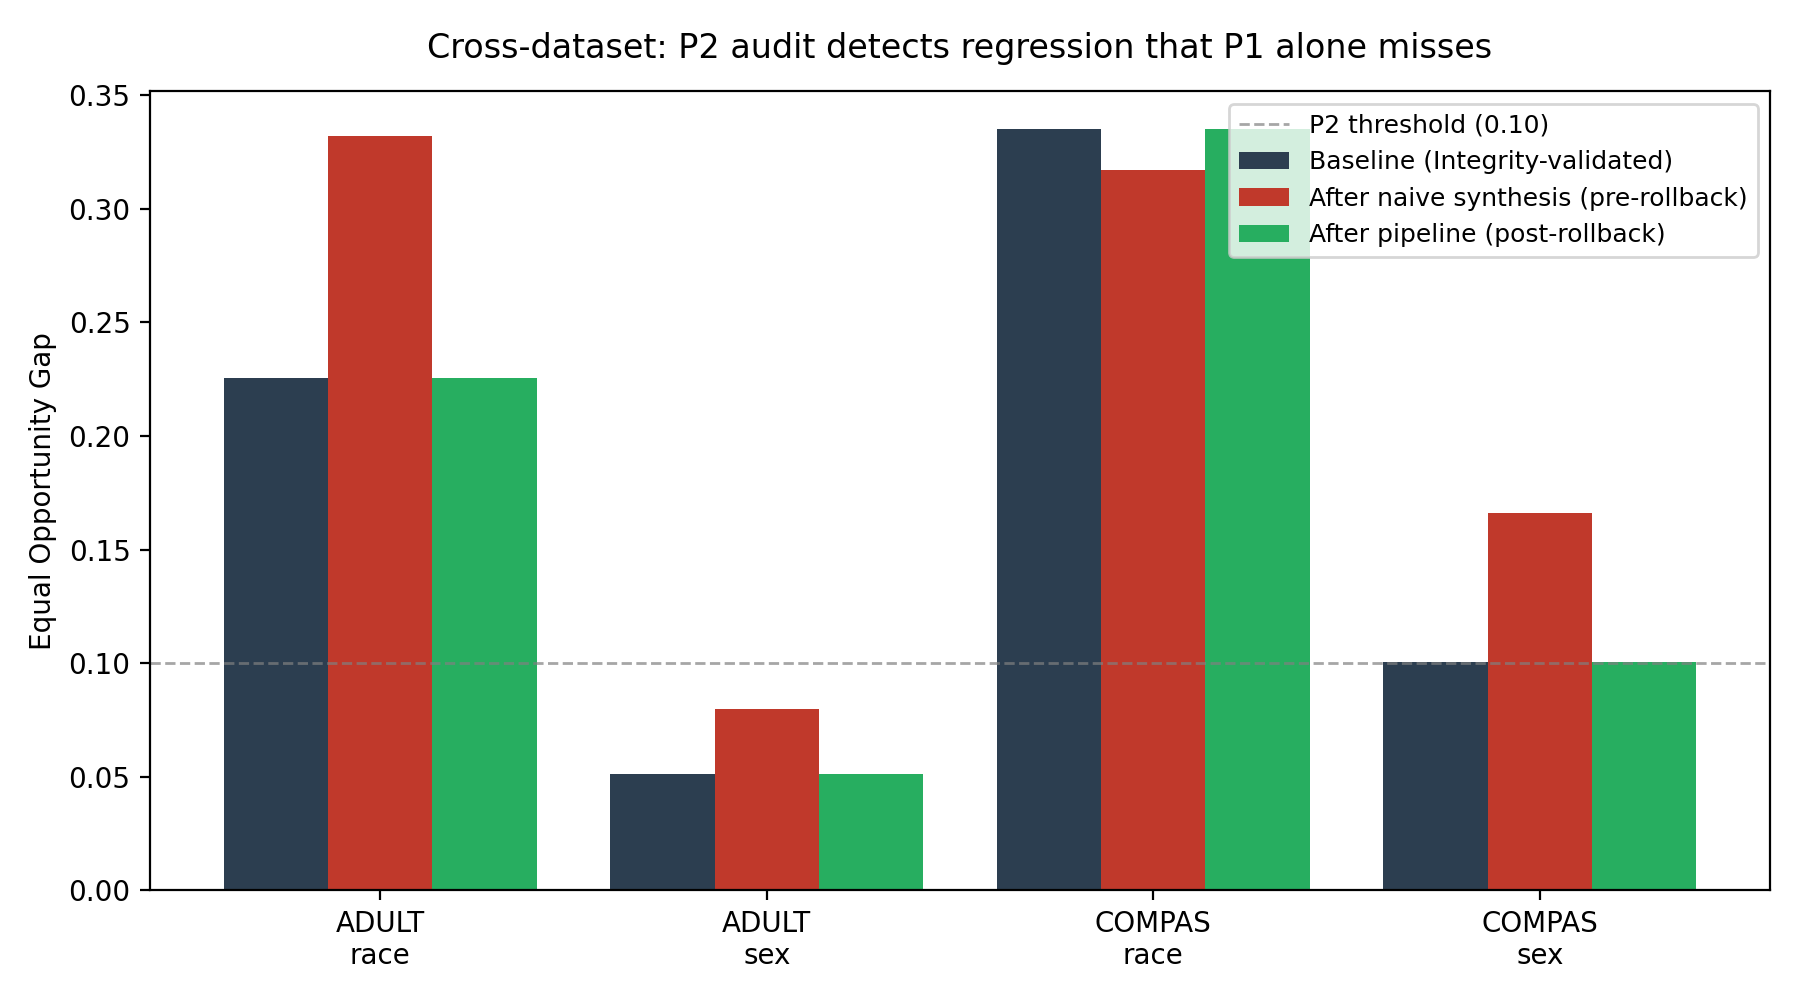
\includegraphics[width=0.9\linewidth]{results/figures/cross_dataset_summary.png}
\caption{Cross-dataset comparison of equal opportunity gap across three states. Baseline (Integrity-validated corpus, navy), after naive synthesis pre-rollback (red), and after pipeline post-rollback (green). The horizontal dashed line marks the P2 threshold (0.10). Naive synthesis worsened the gap on Adult (race: 0.225 $\to$ 0.332; sex: 0.051 $\to$ 0.080), partially improved race on COMPAS (0.335 $\to$ 0.317) but substantially worsened sex (0.100 $\to$ 0.166), and the pipeline's automatic rollback restored the baseline in both cases.}
\label{fig:crossdataset}
\end{figure}

These findings have a specific interpretation. The synthesizer faithfully reproduced the source marginal distribution of each underrepresented group (this is what high P1 confirms; P1 is a marginal-distribution test and does not directly measure joint-dependency fidelity --- a generator can match marginals while distorting feature dependencies, which an extended multivariate P1 metric would catch). Reproducing the marginals of a group whose attribute-target relationship is already biased \emph{amplifies} that bias rather than correcting it: more records of an underrepresented group whose positive-outcome rate is lower than the majority's reinforces the classifier's existing pattern. This is consistent with the conceptual critique of Capasso \cite{Capasso2025}, who argues that synthetic records are epistemic artifacts shaped by the source distribution's existing asymmetries, and with the empirical observation of Kapania et al.\ \cite{Kapania2025} that synthetic data deployed across the AI development pipeline frequently propagates rather than corrects source-distribution biases. Pasculli et al.\ \cite{Pasculli2025} situate the same phenomenon within the regulatory landscape for synthetic data in healthcare and drug development; the present results suggest the corresponding technical control needed to operationalize that regulatory framing.

\paragraph{Threshold sensitivity.} The conflict-resolution protocol fires when any protected attribute's post-synthesis equal-opportunity gap exceeds its pre-synthesis value, which is a strict zero-tolerance threshold on the P2 delta. A reviewer might reasonably ask whether the protocol's behavior is fragile to this choice. We can examine that question against the multi-seed data already collected. If the protocol allowed a tolerance of $\tau = 0.02$ before firing (treating small negative deltas as noise), the multi-seed Adult race column ($-0.1273 \pm 0.0191$) would still trigger rollback in all ten seeds; Adult sex ($-0.0330 \pm 0.0135$) would trigger in nine of ten; COMPAS race ($-0.0014 \pm 0.0162$) would trigger in zero seeds; and COMPAS sex ($-0.0290 \pm 0.0159$) would trigger in seven of ten. If the tolerance were raised further to $\tau = 0.05$, Adult race would still trigger in all ten seeds (the smallest magnitude is $0.10$), Adult sex would trigger in zero, and the COMPAS columns would trigger in zero. The Adult-race regression is robust to reasonable tolerance choices; the other three (dataset, attribute) cells are sensitive to where the line is drawn. The zero-tolerance default we use is a conservative choice: the framework will quarantine more synthesis runs than a permissive threshold would, but it will not quietly admit any regression, however small. Operators with different risk tolerances can adjust the comparison function in the Synthesis Layer's configuration; what the framework requires is that the chosen tolerance be a recorded design decision rather than an unstated default, and the AUTHORIZATION provenance node makes that choice auditable. We report the zero-tolerance default as the choice used in this evaluation, not as an empirical claim about which threshold is correct.

\subsection{Provenance Layer: lineage completeness}

Both runs produced complete provenance graphs. Table~\ref{tab:provenance} reports the evaluation criteria across both datasets.

\begin{table}[h]
\centering
\small
\caption{Provenance Layer evaluation criteria across both runs.}
\label{tab:provenance}
\begin{tabular}{lrrr}
\toprule
\textbf{Metric} & \textbf{Adult} & \textbf{COMPAS} & \textbf{Target} \\
\midrule
Total nodes              & 15    & 14    & ---  \\
Lineage completeness     & 1.00  & 1.00  & 1.00 \\
Decision coverage        & 1.00  & 1.00  & 1.00 \\
Max traceability depth   & 10    & 9     & ---  \\
Orphan nodes             & 0     & 0     & 0    \\
Escalation count         & 2     & 1     & ---  \\
Authorization count      & 2     & 2     & ---  \\
\bottomrule
\end{tabular}
\end{table}

Both runs achieved full lineage completeness (every transformation event carries an explicit rationale, flags, or metrics) and full decision coverage (every escalation has a matching authorization with the role, identity, and rationale of the human authorizer). The traceability depth of 9--10 indicates that any leaf node in the graph --- for instance, the final post-rollback fairness audit --- can be traced back through every prior decision. The full COMPAS provenance graph is shown in Figure~\ref{fig:provenance}.

\begin{figure}[h]
\centering
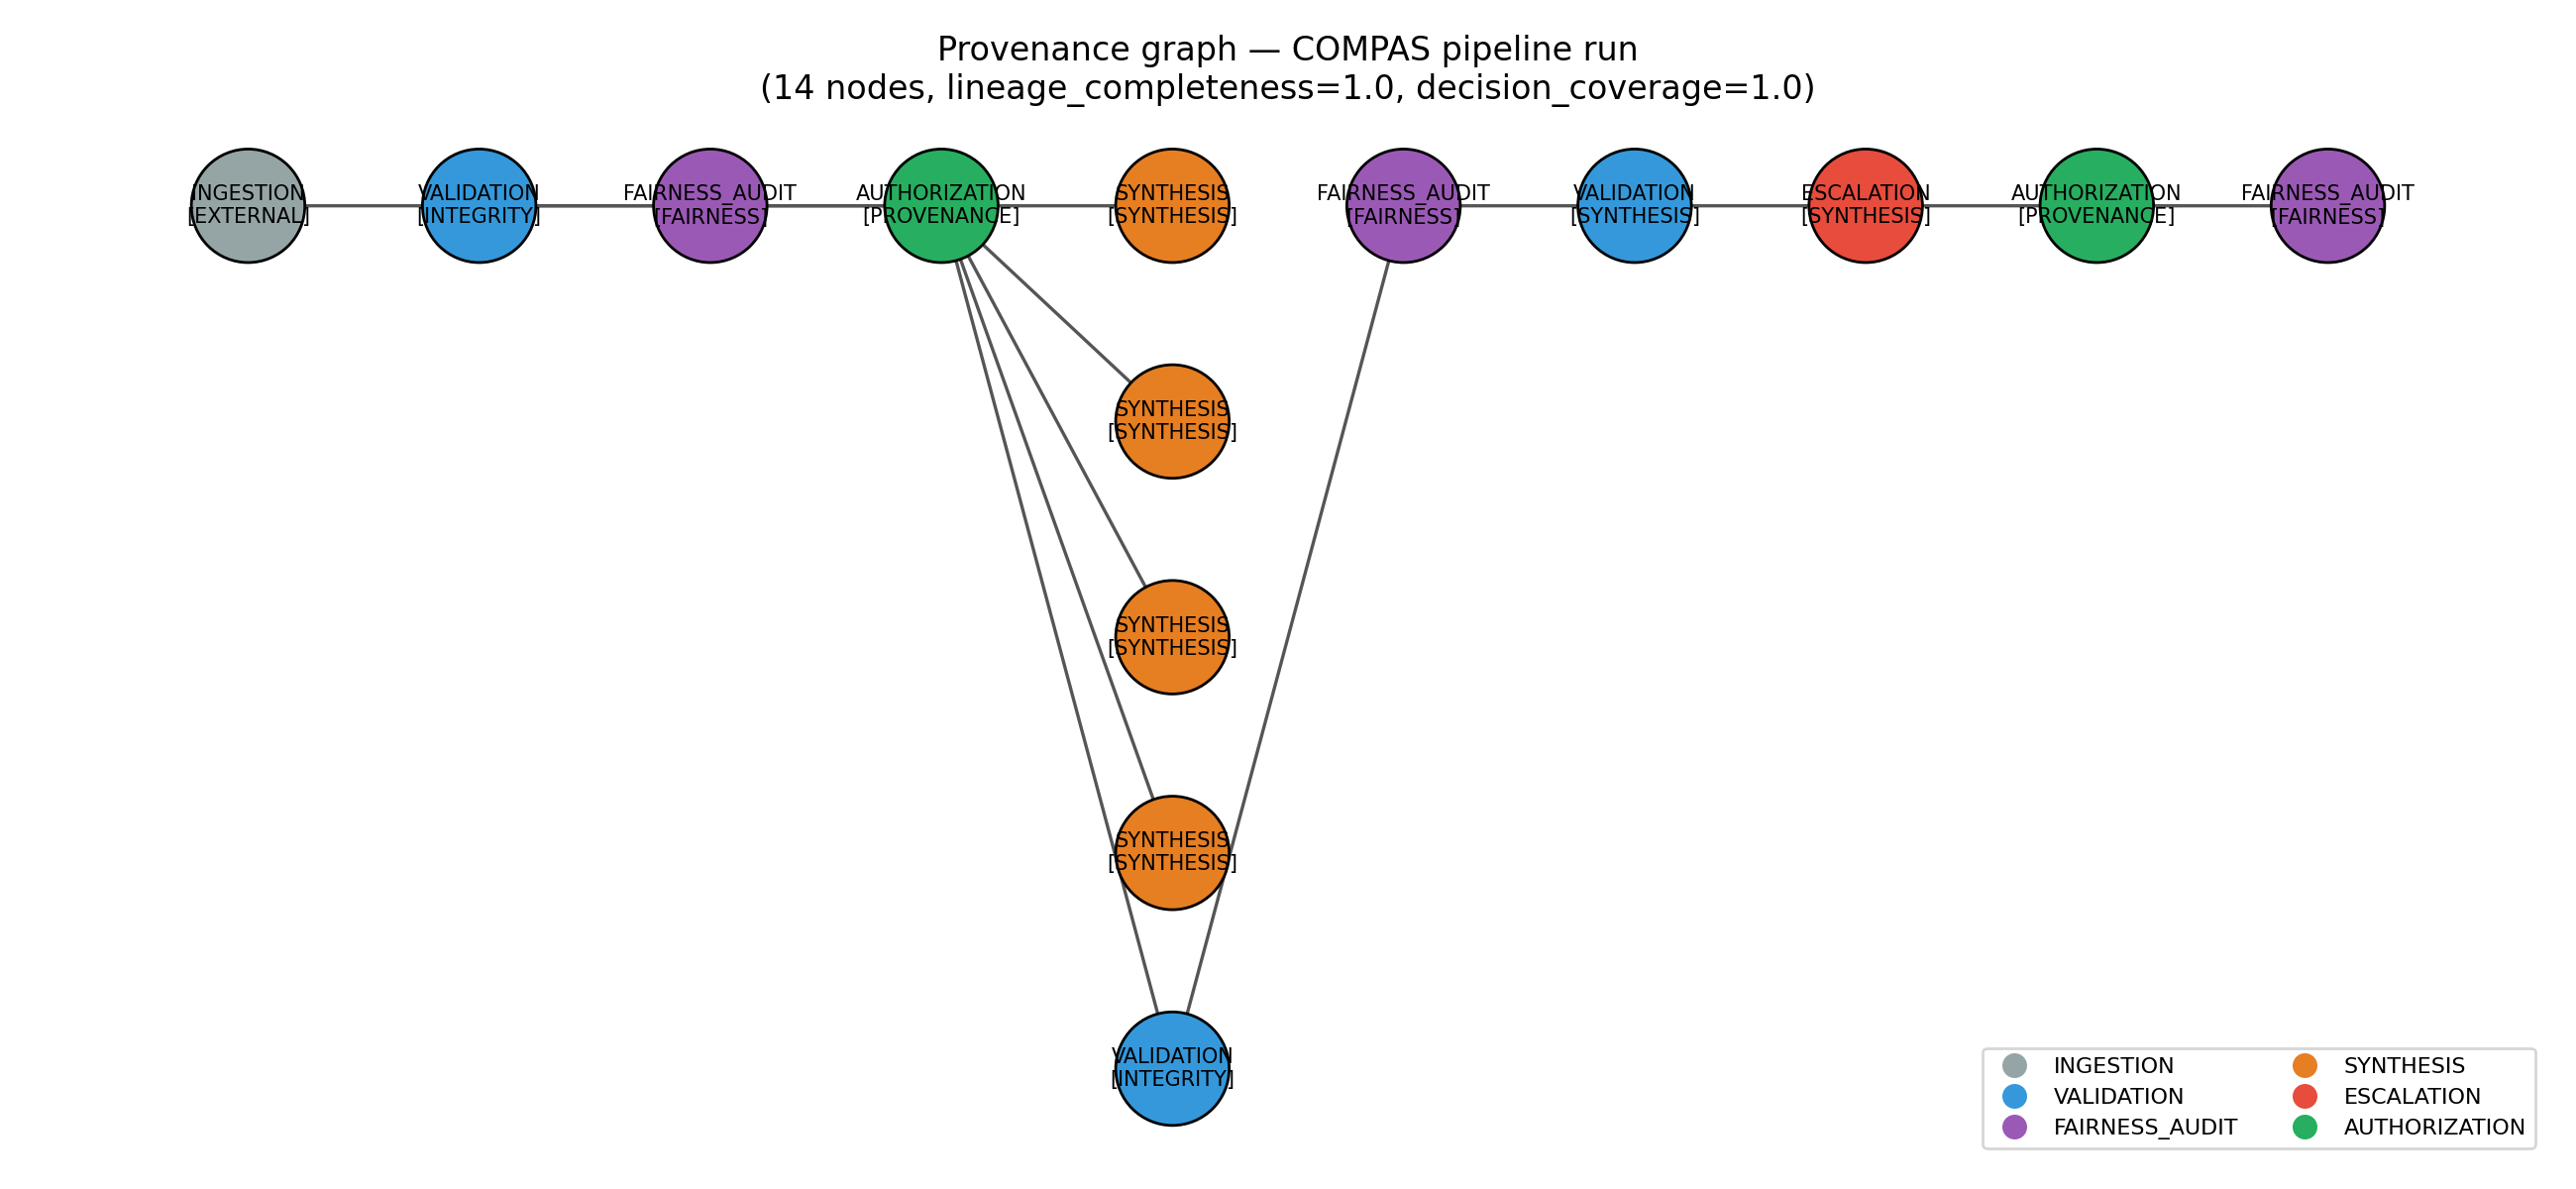
\includegraphics[width=0.95\linewidth]{results/figures/provenance_graph_compas.png}
\caption{Provenance graph for the COMPAS pipeline run. Nodes are color-coded by event type. The flow proceeds from the data source (left) through Integrity validation, initial Fairness audit, Authorization for synthesis, four parallel Synthesis events, Integrity re-validation of the augmented corpus, Fairness re-audit, an Escalation when P2 regression on sex was detected, the Governance Officer's Authorization for rollback, and the final Fairness audit on the rolled-back corpus.}
\label{fig:provenance}
\end{figure}

This is what decision-level provenance means in practice. A regulatory audit of either run can answer not only what changes were made to the training data but who authorized each decision, on what evidence, and with what stated rationale. Specifically, in the COMPAS run, an auditor inspecting the final corpus would find: (i) why 585 synthetic Female records were generated (Fairness Layer detected EO gap of 0.10 on sex); (ii) what cryptographic identifier distinguishes those records from real records (the SHA-256 hash); (iii) why those records were ultimately removed (P2 audit detected $-0.066$ delta on sex); and (iv) who authorized the rollback (the Governance Officer role, with stated rationale). This is the information that post-deployment reviews actually require, and which standard provenance systems do not capture. Across the multi-seed sweep, each pipeline run produced a lineage graph of 13--15 nodes with full lineage and decision coverage, adding well under one second to total execution time.

\subsection{Multi-seed robustness}
\label{subsec:multiseed}

To assess whether the P1-passes-but-P2-fails pattern is an artifact of a single seed or a robust property of the synthesizer-data combination, the full pipeline was run ten times on each dataset with seeds $\{7, 13, 23, 42, 71, 101, 137, 211, 313, 911\}$, holding all other configuration identical. This yields 40 attribute-seed observations (10 seeds $\times$ 2 datasets $\times$ 2 protected attributes). Table~\ref{tab:multiseed} reports the aggregate outcomes.

\begin{table}[h]
\centering
\small
\caption{Multi-seed aggregate outcomes (mean $\pm$ standard deviation across ten seeds). The rightmost column reports how many of the ten seeds produced a negative P2 delta; rollback was triggered in 10/10 seeds for both datasets because at least one protected attribute failed P2 in every seed.}
\label{tab:multiseed}
\begin{tabular}{llcccc}
\toprule
\textbf{Dataset} & \textbf{Attribute} & \textbf{Baseline EO} & \textbf{Pre-rollback EO} & \textbf{P2 $\Delta$} & \textbf{Seeds P2{<}0} \\
\midrule
Adult  & race & $0.2024 \pm 0.0134$ & $0.3297 \pm 0.0180$ & $-0.1273 \pm 0.0191$ & 10 / 10 \\
Adult  & sex  & $0.0532 \pm 0.0106$ & $0.0863 \pm 0.0116$ & $-0.0330 \pm 0.0135$ & 10 / 10 \\
COMPAS & race & $0.3228 \pm 0.0130$ & $0.3242 \pm 0.0113$ & $-0.0014 \pm 0.0162$ &  6 / 10 \\
COMPAS & sex  & $0.0936 \pm 0.0050$ & $0.1226 \pm 0.0169$ & $-0.0290 \pm 0.0159$ & 10 / 10 \\
\bottomrule
\end{tabular}
\end{table}

The pattern that emerges from the multi-seed analysis is more nuanced --- and more diagnostic --- than the single-seed run suggested. On Adult, every seed produced a negative P2 delta on both race (range $-0.1505$ to $-0.1022$) and sex (range $-0.0545$ to $-0.0108$). The seed-42 result reported in the primary run (race $-0.1066$, sex $-0.0286$) sits near the median; the regression is robust to seed variation. On COMPAS, the seed-42 race delta of $+0.0177$ initially appeared to suggest a small but consistent improvement, but at ten seeds the picture changes: the race delta has mean $-0.0014$ (six negative, four positive, range $-0.0290$ to $+0.0298$). The reported single-seed improvement does not generalize; naive Gaussian Copula synthesis on COMPAS race is essentially neutral across seeds, not modestly beneficial. The sex attribute, in contrast, exhibits a consistently negative delta in 10 of 10 seeds (range $-0.0658$ to $-0.0091$). The sex attribute remains the consistent failure point across both datasets. Any positive COMPAS race delta reads as closer alignment with the re-arrest label, which carries its own enforcement biases \cite{Bao2021}, rather than as a substantive reduction of underlying inequity. Figure~\ref{fig:multiseed} displays the per-seed distribution.

\begin{figure}[h]
\centering
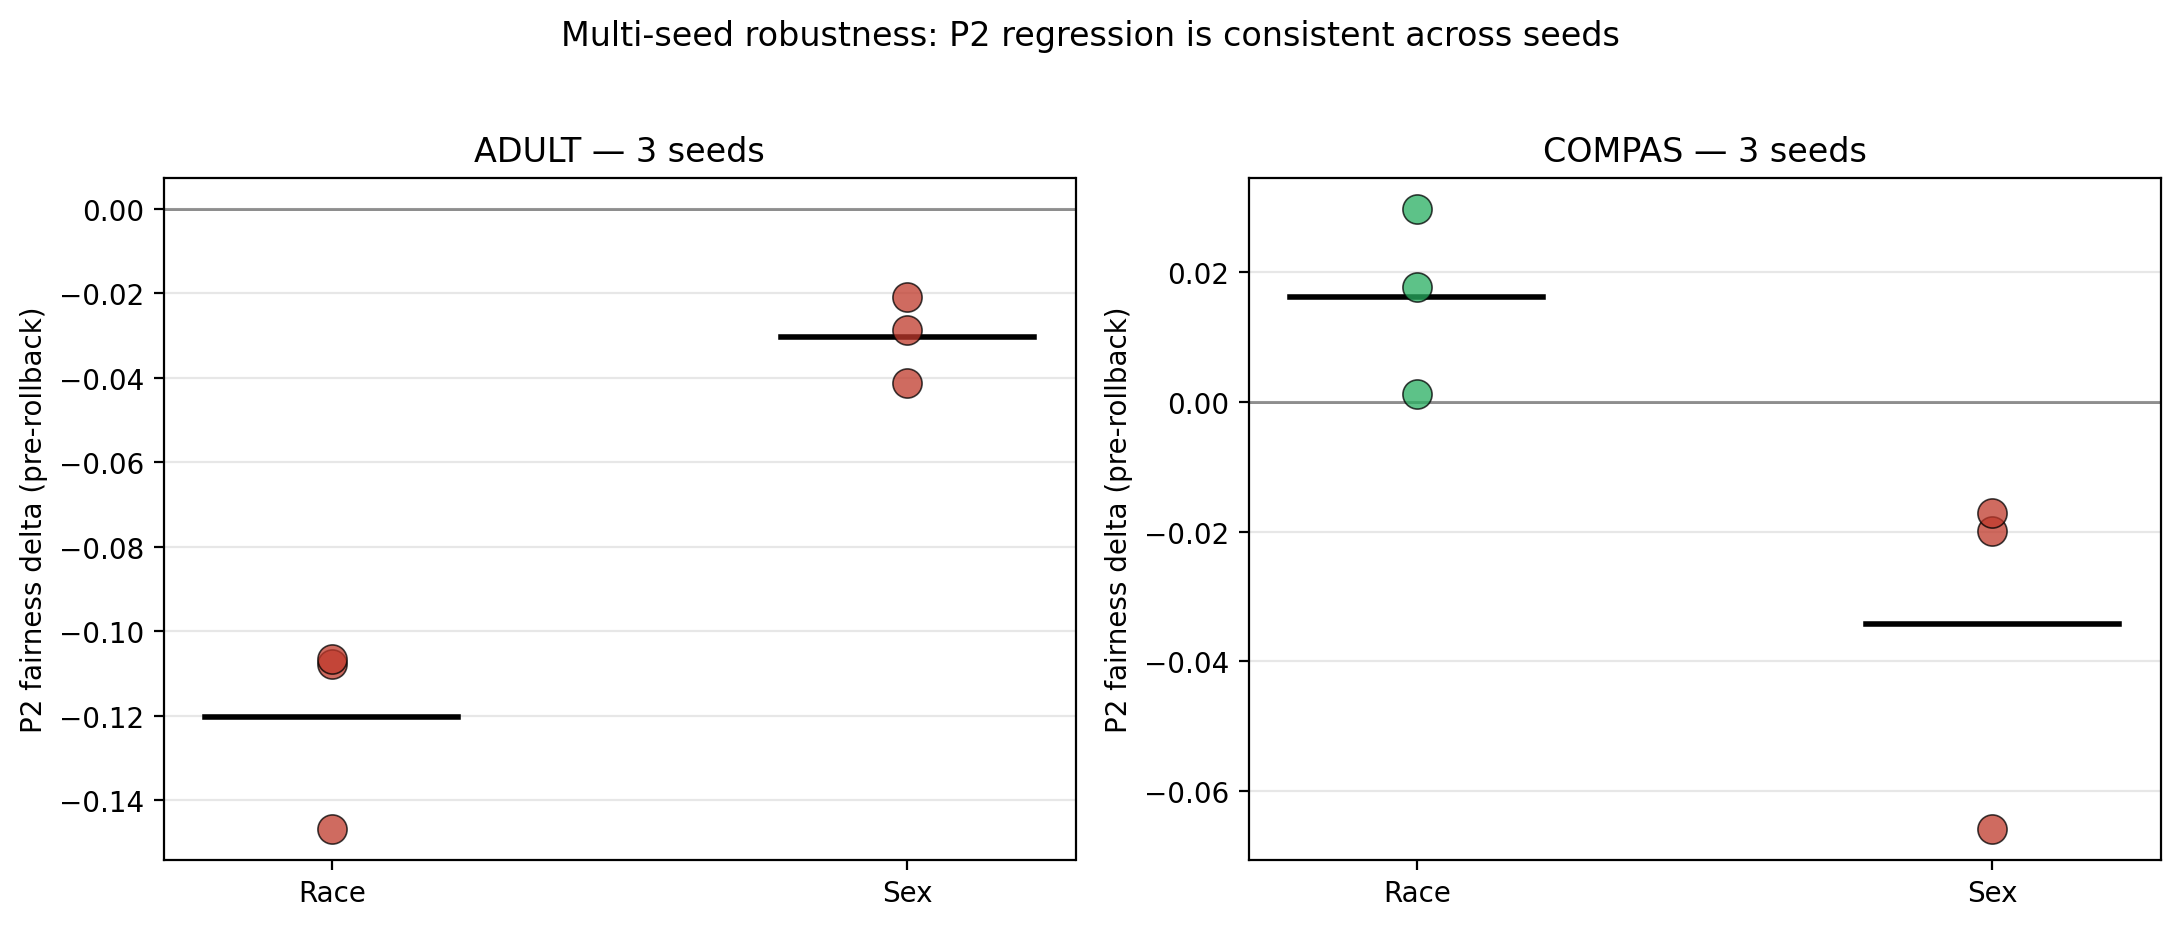
\includegraphics[width=0.95\linewidth]{results/figures/multi_seed_p2_distribution.png}
\caption{Multi-seed robustness of the P2 fairness delta across ten seeds. Each dot is one seed's P2 delta outcome for a given (dataset, attribute) cell; the horizontal black line is the mean across the ten seeds. Red dots correspond to seeds with negative P2 delta (regression); green dots to seeds with non-negative delta. Adult exhibits negative deltas on both attributes across all seeds. COMPAS race exhibits mean $\approx 0$ with six negative and four non-negative seeds; COMPAS sex is negative in all ten seeds. The rollback protocol fired in all 20 (dataset, seed) configurations, since any single negative attribute triggers corpus-level reversion.}
\label{fig:multiseed}
\end{figure}

This result is consequential for the case for naive synthesis. The claim that naive distributional synthesis is sometimes beneficial for fairness does not hold up across seeds: in 36 of 40 attribute-seed observations the P2 delta is non-positive, and the four non-negative outcomes are clustered in a single (dataset, attribute) cell with small magnitudes. \textbf{Across all 20 (dataset, seed) configurations the rollback protocol fired}, because at least one protected attribute failed P2 in every run. The mechanism that surfaces this regression is specifically the joint operation of the batch-level discriminators (P1 detecting distributional drift, P2 detecting the fairness regression) and the Fairness--Synthesis conflict protocol that escalates the result to the rollback decision. In the absence of P2 specifically, an organization running only P1 fidelity checks would have admitted every one of the approximately 80 batches generated by the multi-seed sweep without detecting that, on average, fairness was being preserved or worsened, not improved. P3 and P4, as discussed in Section~\ref{sec:framework}, passed at 100\% across these runs and protect against record-level failures the runs did not produce; the empirical signal here is carried by P1 and P2.

\subsection{Multi-generator robustness}
\label{subsec:multibackend}

To address the concern that the P1-passes-but-P2-fails pattern might be an artifact of the Gaussian Copula's parametric structure, the same pipeline was run with two additional generators of distinct architectural families: CTGAN \cite{Xu2019CTGAN} (a conditional Generative Adversarial Network) and TVAE \cite{Xu2019CTGAN} (a tabular Variational Autoencoder). To keep GAN/VAE training tractable, three seeds shared with the multi-seed analysis $\{13, 42, 137\}$ were used rather than all ten; Adult was subsampled to 5,000 records per run and CTGAN/TVAE were trained for 30 epochs, while COMPAS was used at its full filtered size (6,130 records). The Gaussian Copula values reproduced from Section~\ref{subsec:multiseed} for the three matching seeds appear in Table~\ref{tab:multibackend} as the reference baseline. Figure~\ref{fig:multibackend} displays the per-seed distribution.

\begin{table}[h]
\centering
\small
\caption{Multi-generator aggregate outcomes (mean P2 delta $\pm$ standard deviation across three seeds). P1 pass rate is the fraction of generated batches that passed the distributional invariance check. The P2 column is computed on the subset of seeds where P1 admitted at least one batch into the corpus. Adult runs used a 5,000-record subsample per seed to make CTGAN and TVAE tractable; the Adult Gaussian Copula numbers in Table~\ref{tab:multiseed} use the full dataset.}
\label{tab:multibackend}
\begin{tabular}{llrrcc}
\toprule
\textbf{Dataset} & \textbf{Generator} & \textbf{Attribute} & \textbf{P1 pass rate} & \textbf{P2 $\Delta$} & \textbf{Rollback} \\
\midrule
Adult  & Gaussian Copula & race & 12/12 (100\%) & $-0.1204 \pm 0.0228$ & 3 / 3 \\
Adult  & Gaussian Copula & sex  & 12/12 (100\%) & $-0.0303 \pm 0.0102$ & 3 / 3 \\
Adult  & CTGAN           & race & 9/12 (75\%)   & $+0.0560 \pm 0.0996$ & 3 / 3 \\
Adult  & CTGAN           & sex  & 9/12 (75\%)   & $-0.1388 \pm 0.0153$ & 3 / 3 \\
Adult  & TVAE            & race & 0/12 (0\%)    & undefined            & 0 / 3 \\
Adult  & TVAE            & sex  & 0/12 (0\%)    & undefined            & 0 / 3 \\
\midrule
COMPAS & Gaussian Copula & race & 10/10 (100\%) & $+0.0162 \pm 0.0144$ & 3 / 3 \\
COMPAS & Gaussian Copula & sex  & 10/10 (100\%) & $-0.0343 \pm 0.0273$ & 3 / 3 \\
COMPAS & CTGAN           & race & 10/10 (100\%) & $+0.0156 \pm 0.0395$ & 2 / 3 \\
COMPAS & CTGAN           & sex  & 10/10 (100\%) & $+0.0308 \pm 0.0173$ & 2 / 3 \\
COMPAS & TVAE            & race & 7/10 (70\%)   & $+0.0389 \pm 0.0191$ & 0 / 3 \\
COMPAS & TVAE            & sex  & 7/10 (70\%)   & $+0.0270 \pm 0.0370$ & 0 / 3 \\
\bottomrule
\end{tabular}
\end{table}

\begin{figure}[h]
\centering
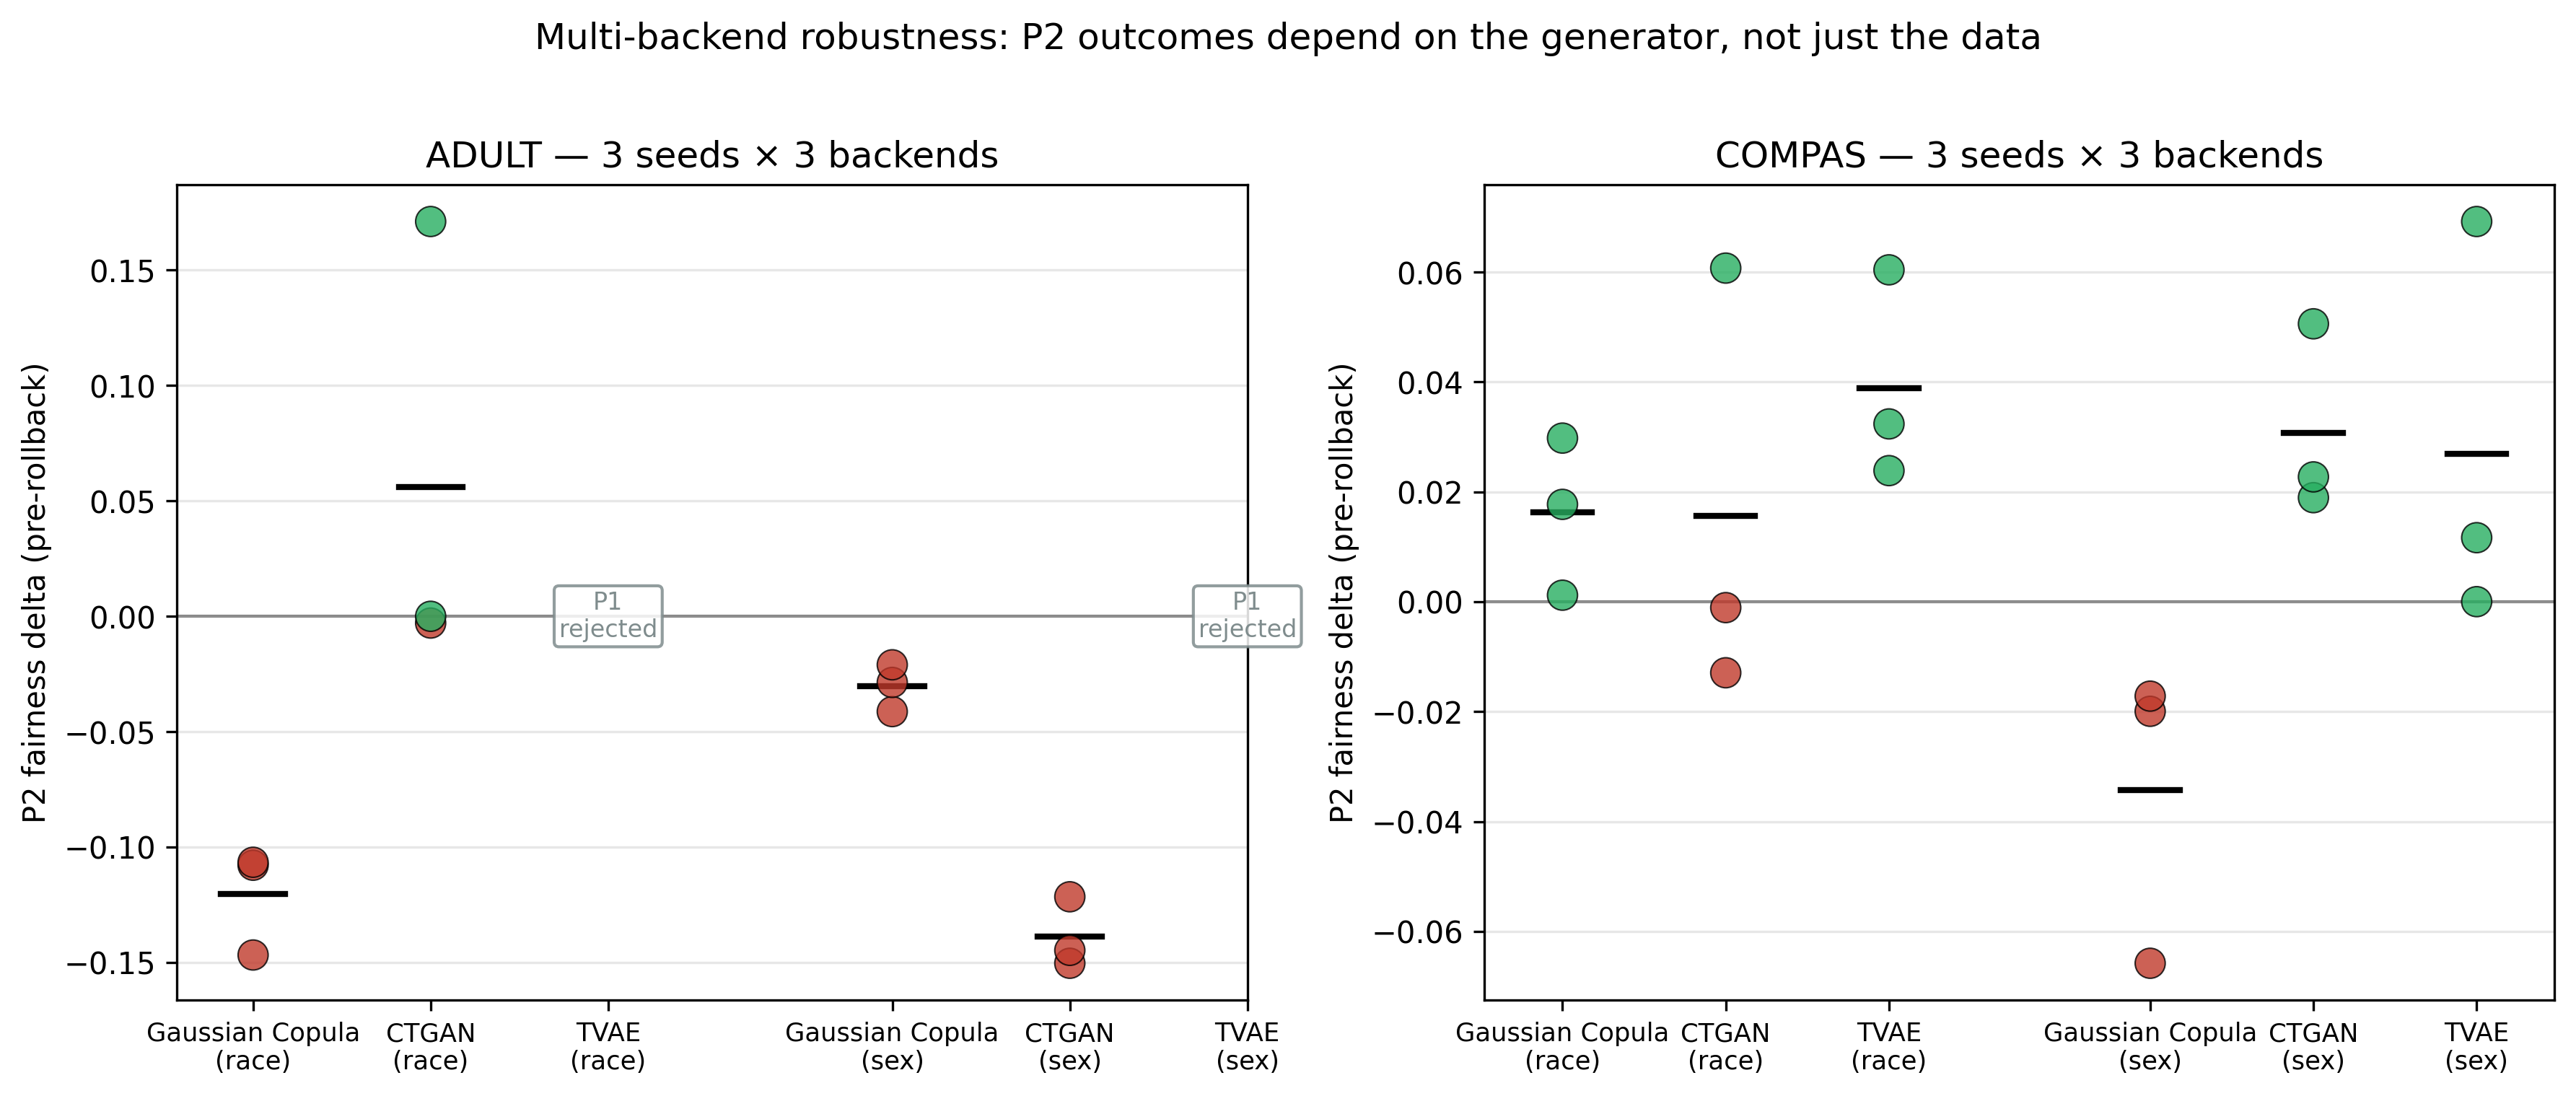
\includegraphics[width=0.95\linewidth]{results/figures/multi_backend_comparison.png}
\caption{Per-seed P2 fairness delta by generator. Each dot represents one (dataset, generator, attribute, seed) cell. The horizontal dashed line marks $P2\Delta = 0$. The three generators produce qualitatively distinct distributions: Gaussian Copula concentrates tightly around small-to-moderate negative deltas; CTGAN produces high-variance outcomes including occasional large positive deltas alongside large negatives; TVAE on COMPAS produces consistently positive deltas, but on Adult it fails P1 entirely and produces no admissible batches at all.}
\label{fig:multibackend}
\end{figure}

The replication yields a richer empirical picture than a simple confirmation of the single-generator finding would. The three generators behave differently across the two datasets in ways that no single protocol alone would detect:

\begin{itemize}[leftmargin=*]
\item \textbf{Gaussian Copula} passes P1 trivially (100\% pass rate on both datasets) but fails P2 on Adult (both attributes, every seed) and on COMPAS sex (every seed). It is the failure mode the single-generator analysis surfaced.

\item \textbf{CTGAN} passes P1 at moderate-to-high rates (75\% on Adult, 100\% on COMPAS) and produces highly variable P2 outcomes by attribute. On Adult race, the three seeds give deltas of $-0.003$, 0.000, and $+0.171$ --- a mean of $+0.056$ that masks two essentially neutral seeds and one strongly positive outlier; on Adult sex, all three seeds give large negative deltas ($-0.150, -0.122, -0.145$), and this sex regression alone triggers rollback in all three Adult runs. On COMPAS, race deltas split into one strongly positive ($+0.061$) and two slightly negative ($-0.013, -0.001$); sex deltas are positive in all three seeds. Rollback fires in two of three COMPAS runs because race, however slightly, regressed in those two seeds.

\item \textbf{TVAE} fails P1 catastrophically on Adult (0\% pass rate; every batch rejected as distributionally implausible) and partially on COMPAS (70\% pass rate, with 1 of 3 seeds admitting only 1 of 3 batches). When TVAE batches do pass P1, they improve fairness on both COMPAS attributes; rollback never fires on COMPAS because no protected attribute regresses in any seed. The Adult TVAE case is the only configuration where P1 functions as a stand-alone gatekeeper, preventing distributionally implausible synthesis from reaching the P2 audit at all.
\end{itemize}

\paragraph{Statistical scope of the multi-generator panel.} The multi-generator analysis is exploratory rather than confirmatory, and we want to be explicit about what that means. Each generator-dataset cell was evaluated at three seeds rather than the ten used in the multi-seed analysis. The reason was tractability: CTGAN and TVAE require gradient-based training that, at ten seeds across two datasets, would have required roughly an order of magnitude more compute time than the copula-based runs. Three consequences follow from this choice and the reader should weight them when interpreting Table~\ref{tab:multibackend}. First, the means we report at $n = 3$ are susceptible to outlier influence in ways that the $n = 10$ multi-seed results are not. The Adult-CTGAN-race column is the clearest case: the reported mean of $+0.056$ aggregates two essentially neutral seeds (deltas of $-0.003$ and $0.000$) and one strongly positive seed (+0.171), and a different choice of three seeds would have produced a substantively different mean. Where we draw qualitative conclusions from the multi-generator panel (which generator passes which protocol, on which dataset), the conclusions are robust to outlier influence because they concern sign patterns and pass rates rather than precise magnitudes; where we report numerical means, the standard deviations should be read as larger than the displayed value suggests. Second, the Adult runs used a per-seed 5{,}000-record subsample to make GAN/VAE training tractable, so the dispersion observed within the Adult-CTGAN and Adult-TVAE rows confounds generator stochasticity with subsample stochasticity. We carry this caveat into the Limitations (Section~\ref{sec:limitations}). Third, the structural argument of this section does not depend on the precise multi-generator magnitudes: it depends on the qualitative observation that different generator families produce qualitatively different failure modes, which would survive even an order-of-magnitude noise floor. A more comprehensive replication, ideally at $n \geq 10$ per generator and including diffusion-based tabular synthesizers, is the natural next step we plan to pursue and report separately.

The empirical findings have a richly diagnostic structure. Across three architecturally distinct generators and ten random seeds, every (dataset, generator) configuration that produced at least one admissible batch also produced at least one protocol failure on at least one protected attribute, and the failure modes differed by generator: Gaussian Copula passed P1 trivially but failed P2; CTGAN passed P1 at moderate rates with high-variance P2 outcomes; TVAE failed P1 entirely on Adult and partially on COMPAS while improving fairness on the batches that did survive P1. No single check would suffice. P1 alone would have admitted the Gaussian Copula's distributionally faithful but fairness-regressing batches; P2 alone would have admitted the TVAE batches whose fairness numbers happened to look acceptable, even though those numbers were computed on synthetic records that bore little resemblance to the source distribution. The Results section connected these patterns to the theoretical critique of synthetic data as an epistemic artifact shaped by the generator's design \cite{Capasso2025,Kapania2025}; the framework's contribution is to make that critique operationally diagnosable. P1 and P2 operating jointly with the conflict-resolution layer above them produce the empirical signal that exposes which kind of failure is occurring. The contribution is not the discovery that any one generator fails; it is the structural specification that catches whichever failure mode is present.

\subsection{The TVAE-on-COMPAS case: governable augmentation under inspection}
\label{subsec:tvae_compas}

One configuration in this evaluation produced an outcome the others did not: TVAE applied to COMPAS led the conflict-resolution protocol to \emph{accept} synthesis rather than reject it. This is, across the 32 dataset-generator-seed configurations covered, the only sustained case of admitted synthetic augmentation, and it deserves more attention than the refusal cases do. The framework's structural argument concerns governance of both refusal and acceptance, but our broader empirical evidence is heavily weighted toward refusal: of the 26 independent pipeline executions, only the three TVAE-COMPAS runs ended without a rollback.

What separates this configuration from the others is the joint behavior of the generator and the dataset. TVAE on COMPAS passed P1 at $7/10$ batches across the three evaluated seeds. On the seven admissible batches, P2 deltas were positive on both protected attributes: race $+0.0389 \pm 0.0191$ and sex $+0.0270 \pm 0.0370$. The same generator on Adult failed P1 catastrophically (every batch rejected). The asymmetry has a candidate explanation. COMPAS, after ProPublica's filtering, has approximately 6{,}130 records and fewer high-cardinality categorical features than Adult; TVAE's variational autoencoder structure, which models a continuous latent distribution and decodes back through a softmax over discrete categorical heads, is more stable on the smaller, more uniformly distributed COMPAS feature space than on Adult's mix of high-cardinality categorical features (occupation, native-country, education) where the decoder's softmax over rare categories collapses. The Gaussian Copula, in contrast, fits parametric marginals and a copula function without trying to learn a latent space, so it passes P1 trivially on both datasets but cannot use that fit to correct fairness regressions. We are not claiming this explanation is settled; it is the hypothesis the data are most consistent with, and a replication with diffusion-based tabular synthesizers (a generator family we did not evaluate) would help test it.

What governance content does an accepted batch carry in our framework that a refused batch does not? Four artifacts. First, the merged corpus retains the synthetic records, each tagged with its SHA-256 hash and source-batch identifier (P3 metadata persists through to the training corpus). Second, the SYNTHESIS provenance node is linked to a downstream VALIDATION node confirming the post-synthesis Integrity re-validation passed --- the recursive verification step of design principle DP1. Third, the AUTHORIZATION node records the role and rationale of the human approver who reviewed the P2 deltas and judged them acceptable; in our run this is the Governance Officer role, with rationale text noting the positive P2 deltas on both protected attributes and the source-distribution justification for accepting the modified TVAE batches. Fourth, the lineage graph carries forward a record of which records are synthetic so that any downstream fairness audit on the deployed model can be re-computed against the real-records-only subset for comparison.

This is the kind of artifact a regulatory audit needs to interrogate an acceptance decision. It does not, in itself, validate the substantive claim that TVAE-on-COMPAS reduces real-world unfairness --- the COMPAS labels themselves encode the enforcement patterns of the criminal justice system \cite{Bao2021}, and a positive P2 delta on race in this dataset reads as closer alignment with the re-arrest label rather than as substantive reduction of injustice (we return to this in Section~\ref{sec:discussion}). What the artifact does is make the acceptance decision \emph{interrogable}: a downstream reviewer can ask which records were added, why, who approved their addition, and what fairness numbers were before and after. The framework's contribution in the accepted-synthesis case is the same as in the refused-synthesis case: a structure for surfacing trade-offs in a form a human can be held responsible for. We do not over-claim from one positive configuration; we record it as the single observation we have of the framework's behavior when synthesis succeeds, and we are explicit that more such observations are needed before the conditions for governable augmentation can be characterized in general.

%=========================================================================
% 4. DISCUSSION
%=========================================================================
\section{Discussion}
\label{sec:discussion}

\paragraph{Comparison with related frameworks.} The Data-Centric Trust Pipeline is positioned alongside but distinct from the data-centric perspective of Dammu et al.\ \cite{Dammu2026}, who propose a layered structure integrating governance, fairness, validation, and lifecycle accountability. The differences are substantive rather than presentational. The framework we propose formalizes the inter-layer dependencies that a purely layered description leaves implicit --- through a taxonomy of inputs, outputs, and explicit conflict-resolution protocols. Consider what this buys concretely: in our framework, an integrity exclusion that disproportionately removes underrepresented records is detected by the Integrity Layer's demographic coverage parity check, raised as an Integrity--Fairness conflict, and routed to human authorization \emph{before} the records are dropped, with the rationale recorded as a lineage node. A layered framework without specified inter-layer protocols treats demographic completeness as a downstream fairness concern, surfacing it only after model evaluation when the harm is harder to attribute. Beyond this, synthetic data in our work is a first-class governance layer with its own validation structure rather than a bias-mitigation add-on, and the empirical demonstration grounds the framework in measurable artifacts (provenance graphs, per-batch protocol outcomes, rollback decisions) rather than in conceptual claims alone. Relative to the NIST AI RMF \cite{NIST_AIRM_2023} and ISO/IEC 42001 \cite{ISO_42001_2023}, the pipeline is more granular at the data layer but compatible with their organizational scope --- those frameworks tell an organization \emph{what} to document; we describe one architecture for generating that documentation as a side effect of the data workflow itself.

\paragraph{Relationship to class-balancing methods.} A natural question is whether the present results merely repeat what SMOTE-style oversampling already establishes \cite{Chawla2002SMOTE}. They do not, and the difference is informative. SMOTE oversamples the minority \emph{class}; the Synthesis Layer oversamples the underrepresented protected \emph{group}, with the source distribution of that group as its generation prior --- this is a different intervention, but not the substantive distinction. The substantive distinction is that the contribution of this work is not the generator at all. It is the validation structure surrounding the generator. The same P1 and P2 protocols applied to SMOTE-generated records would yield the same conclusion --- high distributional fidelity, potential P2 failure when the underlying attribute-target relationship is itself biased --- because the failure mode lives in the source distribution, not in the synthesizer. What makes the synthesis governable in our framework is the protocol audit, the cryptographic per-record provenance, the corpus-level P2 evaluation across all protected attributes jointly, and the conflict-resolution rollback. Any tabular synthesizer that exposes a \texttt{fit}/\texttt{sample} interface can plug into the Synthesis Layer's backend; the structure that catches the failure mode is upstream of the choice of generator.

\paragraph{Implications for regulation.} The EU AI Act, ISO/IEC 42001, and the NIST AI RMF all specify what must be documented: datasets must be characterized, training procedures recorded, post-deployment monitoring established. None of them specifies how those category-level requirements relate to one another in practice. An organization can satisfy every documentation requirement of the EU AI Act with a static data card describing the synthetic batches generated in this evaluation, and still operate a pipeline in which the P2 regression we measured would go undetected: the data card lists what is in the dataset, not whether the fairness audit ever ran against the synthetic records, not who authorized their inclusion, not what they were rebalancing for. The regulatory framing this work suggests is a shift from entity-level accountability --- which organization is responsible? --- to decision-level accountability: which decision, made by whom, on what evidence, produced this outcome? The minimum lineage record described in Section~\ref{sec:framework} is one concrete proposal for what such a regime would require operationally. It will not, by itself, solve the harder political question of who has standing to interrogate those records; that question sits in front of, not behind, the technical work.

\paragraph{Rollback preserves the baseline; it does not correct bias.} A central interpretive caveat: when the conflict-resolution protocol fires and the pipeline rolls a synthesis attempt back, the result is a return to the baseline disparity, not a reduction of it. The Adult race equal-opportunity gap remains at 0.225 after rollback; the COMPAS race gap remains at 0.335. The Pipeline does not claim to make the world more equitable through synthesis. What it does is refuse to make matters worse through unaudited augmentation, and it documents that refusal in a way that downstream actors --- regulators, ethics boards, affected communities --- can interrogate. A naive read of the framework could license inaction (``the Pipeline rejected the augmentation, so the bias is not our responsibility''); a faithful read makes the opposite move (``the Pipeline made visible that this generator cannot reduce the bias, so the responsibility now sits with a deliberate human decision about what intervention to attempt next''). The Pipeline is a substrate for accountable choice among interventions; it is not a substitute for choosing.

\paragraph{Scope conditions and what the pipeline does not do.} The pipeline is designed for AI systems where demographic disparities in outcomes carry significant ethical, legal, or clinical weight --- the sensitive domains identified in the Introduction. It is less directly applicable to settings where training data does not involve person-level records or where the primary risk is not distributional bias but model robustness or adversarial vulnerability. The framework governs the data layer; model-level fairness interventions (e.g., adversarial debiasing, post-hoc calibration) are complementary rather than substitutable, and would be triggered by the framework's authorization records as separate downstream interventions rather than absorbed into the data pipeline.

\subsection{Limitations}
\label{sec:limitations}

Four limitations bound the empirical claims.

First, although the multi-generator analysis covered three architectural families (copula-based parametric, generative adversarial network, and variational autoencoder), it did not include diffusion-based tabular synthesizers, which have emerged as a separate generative family with distinct distributional behavior. The framework's design is synthesizer-agnostic --- any tabular generator that conforms to the \texttt{fit}/\texttt{sample} interface can be plugged in --- but the specific quantitative findings reported here are conditional on the three generators evaluated. Replication with diffusion-based generators is a natural extension and the implementation supports straightforward backend addition.

Second, the evaluation uses Adult and COMPAS --- canonical but small fairness benchmarks with documented limitations \cite{Bao2021}. The framework's behavior on larger-scale industrial pipelines, particularly with many more protected attributes or with intersectional groupings, remains to be tested. The expectation is that the inter-layer protocols scale (their cost is constant per transformation event), but the human-escalation paths require organizational infrastructure that not all settings provide.

Third, the framework presumes organizational conditions that are not universal. It expects defined roles --- a Data Steward, a Fairness Analyst, a Governance Officer --- a shared semantic ontology for cross-source validation, and provenance records held as institutional artifacts with retention and access policies attached to them. Implemented in their absence, the technical components produce documentation that is filled in but not interpretively meaningful. A subtler failure mode, which the framework cannot eliminate from within, is the degradation of the human authorization step into a rubber stamp: a Governance Officer who approves every rollback (or every override) without engaging the trade-off would meet the protocol's literal requirement while hollowing out its accountability content. We can mitigate this only partially. The AUTHORIZATION provenance nodes carry the actor's identity, the rationale text, and the timestamp, and a downstream review can mine those records for the patterns that betray rote approval --- boilerplate rationale, short decision turnaround, weak alignment between the stated rationale and the flag that surfaced the decision. What we cannot specify in code is the institutional process that converts those records into a serious evaluation of the human judgment they document. That process is a precondition for the framework's accountability claim, and we want to be honest that it is not something the framework itself delivers.

Fourth, a handful of methodological choices shape the specific numbers we report without changing the qualitative finding that no single protocol detects every failure mode. The Fairness Layer's audit classifier is a random forest, which is one choice among several. To check whether the P2 sign pattern was an artifact of that choice, we re-ran the three multi-seed seeds (13, 42, 137) on both datasets with a logistic regression classifier substituted in. The sign pattern survived: Adult race $-0.058$, Adult sex $-0.077$, COMPAS race $+0.011$ (still essentially neutral), COMPAS sex $-0.062$. Magnitudes shift, the qualitative pattern does not, and the ablation data are released as \texttt{classifier\_ablation\_raw.csv} alongside the rest of the code. The multi-generator Adult runs used a per-seed 5{,}000-record subsample to keep CTGAN and TVAE training tractable, which means the Adult variance figures for those generators conflate generator stochasticity with subsample stochasticity --- this is a known limit of the design we did not separately disentangle, and the COMPAS multi-generator runs and the full multi-seed Adult sweep with Gaussian Copula are free of that confound. Finally, the P4 plausibility rules used here are illustrative range checks rather than serious deployment-grade rules. Production deployments would want richer co-occurrence constraints (for instance, that hours-per-week of zero is inconsistent with a non-trivial occupation), which the framework supports through arbitrary callable predicates; we did not invest in elaborating these rules because they did not bear on the structural argument of this article.

%=========================================================================
% 5. METHODS / REFERENCE IMPLEMENTATION
%=========================================================================
\section{Methods}
\label{sec:methods}

\subsection{Implementation}

The pipeline is implemented in Python 3.12 across five modules: \texttt{integrity.py}, \texttt{fairness.py}, \texttt{synthesis.py}, \texttt{provenance.py}, and \texttt{pipeline.py}, totalling approximately 1,560 lines. Dependencies include \texttt{pandas}, \texttt{numpy}, \texttt{scipy}, \texttt{scikit-learn}, \texttt{fairlearn}, \texttt{sdv} (which provides the Gaussian Copula, CTGAN, and TVAE synthesizers used in the empirical evaluation), and \texttt{networkx} (lineage graph). The full implementation is open-source under the MIT License; the public release contains pinned dependency versions and single-command reproduction scripts.

\subsection{Datasets}

Adult Census Income was obtained from the \texttt{algofairness/fairness-comparison} GitHub mirror of the UCI repository (32,561 records, 15 columns). COMPAS Recidivism was obtained from the \texttt{propublica/compas-analysis} GitHub repository (7,214 records, 53 columns; reduced to 6,130 after standard filtering). Both are publicly available; neither contains personally identifiable information beyond what the original sources released.

\subsection{Configuration}

The configuration used for all empirical runs:
\begin{itemize}[leftmargin=*, itemsep=1pt]
  \item Random state: 42 for the primary single-seed run.
  \item Fairness Layer thresholds: equal-opportunity gap $\leq 0.10$; underlying classifier is a random forest (100 estimators, max depth 10).
  \item Synthesis Layer thresholds: P1 Jensen--Shannon divergence threshold of 0.10; P4 minimum plausibility pass rate of 0.95; oversampling ratio of 0.5, capped at 3,000 records per group.
  \item Gaussian Copula configuration (SDV defaults): enforce min/max values; do not enforce rounding.
  \item Counterfactual fairness sampling: 500 records, 1-nearest neighbor matching across the opposite protected-attribute group.
  \item Multi-seed analysis (Section~\ref{subsec:multiseed}): ten seeds $\{7, 13, 23, 42, 71, 101, 137, 211, 313, 911\}$, holding all other parameters constant.
  \item Multi-generator analysis (Section~\ref{subsec:multibackend}): three of those seeds $\{13, 42, 137\}$. CTGAN and TVAE on COMPAS used 150 training epochs on the full filtered dataset; on Adult the same generators used 30 epochs on a per-seed 5,000-record subsample.
\end{itemize}

\subsection{Per-record cryptographic provenance (P3)}

Each synthetic record's identity hash is computed as
\[
\mathrm{SHA256}(\text{model\_id} \mid \text{batch\_id} \mid \text{record\_idx} \mid \text{seed} \mid \text{timestamp\_iso}),
\]
attached as the \texttt{\_\_provenance\_hash} column at generation time, and the batch hash set is registered as a SYNTHESIS node in the Provenance Layer before the batch is released. Verification at integration time checks both hash well-formedness (64 hex characters) and within-batch uniqueness.

\subsection{Plausibility rules (P4)}

Domain rules are passed as callables that evaluate a single record. For Adult: \texttt{age} $\in [17, 90]$, \texttt{hours-per-week} $\in [1, 99]$, \texttt{education-num} $\in [1, 16]$. For COMPAS: \texttt{age} $\geq 17$, \texttt{priors\_count} $\geq 0$, \texttt{decile\_score} $\in [1, 10]$. These are illustrative defaults; production deployments should derive rules from domain expert validation as specified in the framework.

\subsection{Reproducibility}

The complete reproduction sequence is:

\begin{verbatim}
pip install -r requirements.txt
python experiments/run_adult.py
python experiments/run_compas.py
python experiments/cross_dataset.py
# Multi-seed robustness:
for seed in 7 13 23 42 71 101 137 211 313 911; do
    python experiments/single_seed.py --dataset adult  --seed $seed
    python experiments/single_seed.py --dataset compas --seed $seed
done
python experiments/aggregate_multi_seed.py
# Multi-generator robustness:
for seed in 13 42 137; do
  for backend in ctgan tvae; do
    python experiments/single_backend.py --dataset compas --seed $seed \
        --backend $backend --epochs 150
    python experiments/single_backend.py --dataset adult --seed $seed \
        --backend $backend --epochs 30 --adult-sample 5000
  done
done
python experiments/aggregate_multi_backend.py
# Classifier ablation:
python experiments/classifier_ablation.py
\end{verbatim}

All artifacts (per-run JSON summaries, provenance graphs, figures, comparison tables) regenerate deterministically. Total wall-clock time on commodity hardware is approximately 60--75 minutes including all replication sweeps.

%=========================================================================
% ACKNOWLEDGMENTS
%=========================================================================
\section*{Acknowledgments}

This research was conducted as part of the author's extended research and residency activities at the Sloan School of Management within the Visiting Fellows Program at the Massachusetts Institute of Technology (MIT). The author, a professor and researcher at the CESAR School (Recife Center for Advanced Studies and Systems), gratefully acknowledges the academic environment and interdisciplinary dialogue that supported the intellectual development of this study. The author also thanks the two anonymous reviewers and the editors of \textit{AI and Ethics} for the detailed and constructive feedback that materially improved this manuscript.

%=========================================================================
% STATEMENTS AND DECLARATIONS
%=========================================================================
\section*{Statements and Declarations}

\paragraph{Funding, competing interests, and consent.} This research received no external funding, and the author declares no competing interests. The study uses only publicly released secondary datasets and generated no new data from human subjects, so institutional ethics review and consent to participate were not engaged --- this is the standard treatment for secondary-data analysis of pre-existing public benchmarks. Consent for publication is not applicable for the same reason.

\paragraph{Data availability.} The empirical evaluation draws on two publicly available datasets, both redistributed verbatim in the public code release under their original licenses.

\begin{itemize}[leftmargin=*, itemsep=2pt]
\item \textbf{Adult Census Income} (also called ``Census Income''), available from the UCI Machine Learning Repository at \url{https://doi.org/10.24432/C5XW20}, licensed CC BY 4.0, originally compiled by Becker and Kohavi (1996) \cite{Becker1996Adult}.
\item \textbf{ProPublica COMPAS Recidivism} (\texttt{compas-scores-two-years.csv}), released by ProPublica alongside Angwin, Larson, Mattu, and Kirchner's ``Machine Bias'' (2016), available at \url{https://github.com/propublica/compas-analysis}. No DOI exists for this dataset; the GitHub repository URL is its canonical persistent reference \cite{ProPublica2016COMPAS}.
\end{itemize}

\paragraph{Code availability.} The reference implementation --- five framework modules, experiment scripts, configuration files, the generated provenance graphs, and the tabulated outcomes --- is released under the MIT License at \url{https://github.com/cdiegocom/dctp}. The version of record corresponding to this manuscript is tagged \texttt{v1.0.0} in that repository.

\paragraph{Author contributions (CRediT).} \textbf{Carlos Diego Cavalcanti Pereira}: Conceptualization, Methodology, Software, Validation, Formal analysis, Investigation, Resources, Data curation, Writing -- original draft, Writing -- review \& editing, Visualization, Project administration.

\paragraph{Use of generative AI tools.} This manuscript was prepared with the assistance of a large language model used for copy editing (improvements to grammar, spelling, punctuation, and style of human-written text) and for code review assistance during implementation. The conceptual framework, experimental design, empirical findings, interpretation of results, and final manuscript content are the work of the author. No portion of the manuscript text or the substantive analysis was generated autonomously by an AI system. This use is consistent with Springer Nature's policy on AI-assisted writing and authorship; LLMs are not listed as authors.

%=========================================================================
% REFERENCES
%=========================================================================
\begingroup
\sloppy
\printbibliography
\endgroup

\end{document}
